\section{XML Processing} 
\hspace*{0.5in} XML adalah bahasa open source portable yang mungkinkan pemrogram mengemangkan aplikasi yang dapat dibaca oleh aplikasi lain, terlepas dari sistem operasi dan bahasa pengembangnya. 
\vspace{12pt}
 
\hspace*{0.5in} Extensible Markup Languange (XML) adalah bahasa markup seperti HTML atau SGML. Ini direkomendasikan oleh World Wide Web Consortium dan tersedia sebagai standar terbuka. XML sangat berguna untuk mencatat data berukuran kecil dan menengah tanpa memerlukan tulang punggung berbasis SQL. 

\vspace{12pt}
\subsection{Arsitektur Parsing XML dan API} 
 
\hspace*{0.5in} Perpustakaan standar Python menyediakan seperangkat antarmuka minimal tapi berguna untuk bekerja dengan XML.  
 
\hspace*{0.5in} Dua API yang paling dasar dan umum digunakan untuk data XML adalah antarmuka SAX dan DOM. 
 
\hspace*{0.5in} API sederhana untuk XML (SAX): mendaftarkan panggilan kemali untuk acara yang diminati dan kemudian membiarkan parser berjalan melalui dokumen. Ini berguna bila dokumen berukuran besar atau memiliki keterbatasan memori, ini memparsing file tidak pernah tersimpan dalam memori. 
 
\hspace*{0.5in} API Document Objek Model (DOM): ini adalah rekomendasi World Wide Web Consortium dimana keseluruhan file dibaca ke memori dan disimpan dalam bentuk hierarkies (tree-based) untuk mewakili semua fitur dokumen XML.  
 
\hspace*{0.5in} SAX jelas tidak bisa memproses informasi secepat DOM saat bisa bekerjadengan file besar. Di sisi lain, menggunakan DOM secara eklusifenar-benar dapat membunuh sumber daya, terutama jika digunakan pada banyak file kecil. 
 
\hspace*{0.5in} SAX hanya bisa dibaca sementara DOM mengizinkan perubahan pada file XML. Kedua API yang berbeda ini saling melengkapi satu sama lain, tidak ada alasan mengapa tidak dapat menggunakannya untuk proyek besar. 
\vspace{12pt}
 
Contoh: 
\begin{verbatim} 
<collection shelf="New Arrivals"> 
 
<movie title="Enemy Behind"> 
 
    <type>War, Thriller</type> 
 
    <format>DVD</format> 
 
    <year>2003</year> 
 
    <rating>PG</rating> 
 
    <stars>10</stars> 
 
    <description>Talk about a US-Japan war</description> 
 
</movie> 
 
<movie title="Transformers"> 
 
    <type>Anime, Science Fiction</type> 
 
    <format>DVD</format> 
 
    <year>1989</year> 
 
    <rating>R</rating> 
 
    <stars>8</stars> 
 
    <description>A schientific fiction</description> 
 
</movie> 
 
    <movie title="Trigun"> 
 
    <type>Anime, Action</type> 
 
    <format>DVD</format> 
 
    <episodes>4</episodes> 
 
    <rating>PG</rating> 
 
    <stars>10</stars> 
 
    <description>Vash the Stampede!</description> 
 
</movie> 
 
<movie title="Ishtar"> 
 
   <type>Comedy</type> 
 
   <format>VHS</format> 
 
   <rating>PG</rating> 
 
   <stars>2</stars> 
 
   <description>Viewable boredom</description> 
 
</movie> 
</collection>
\end{verbatim}
 
\vspace{10pt}
\subsection{Parsing XML dengan API SAX} 
 
\hspace*{0.5in} SAX adalah antarmuka standar untuk parsing XML berbasis event. Parsing XML dengan SAX umumnya mengharuskan untuk membuat C\textit{ontrolHandler }dengan subclassing xml.sax \textit{controlhandler}. 
 
\hspace*{0.5in} \textit{ControlHandler }menangani tag dan atribut tertentu dari XML. Objek \textit{ControlHandler }menyediakan metode untuk menangani berbagai aktivitas parsing. Parsing memanggil metode \textit{ControlHandler }saat memparsing file XML. 

\hspace*{0.5in} Metode \textit{startDocument} dan \textit{endDocument} disebut awal dan akhir setiap elemen. Jika parsing tidak dalam mode namespace, metode \textit{startElement} (tag attribute) dan \textit{endElement} (tag) dipanggil. Jika tidak, metode yang sesuai \textit{startElemenNS} dan \textit{endElemenNS} dipanggil. Disini, tah adalah tag elemen dan atribut adalah atribut.  
 
\hspace*{0.5in} Metode-metode berikut membuat objek parsing baru dan mengembalikannya. Objek parsing diuat akan menjadi tipe parsing pertama yang ditemukan sistem.  
{\fontsize{10pt}{10pt}\selectfont xml.sax.make $  \_  $parser([parser $  \_  $list])} .Parameter 
Parser $  \_  $list pilihan argumen yang terdiri dari daftar parsing untuk digunakan yang semuanya harus menerapkan metode \textit{make $  \_  $parse} 
 
\hspace*{0.5in} Metode-metode berikut membuat parsing SAX dan menggunakannya untuk mengurai dokumen {\fontsize{10pt}{10pt}\selectfont xml.sax.parser(xmlfile, contenthandler[, errorhandler])}. Berikut adalah detail dari parameternya: 
 
\begin{itemize}
\item \textit{Xmlfile } 

Ini adalah nama file XML yang bisa dibaca. 
\item \textit{ContentHandler } 

Ini harus menjadi objek \textit{ContenHandler} 
\item \textit{ErrorHandler} 

Jika ditentukan, e\textit{rrorhandler} harus menjadi objek \textit{ErrorHandler} SAX 
\item Metode\textit{ parseString}
\end{itemize}

\vspace{12pt} 
Membuat parsing SAX dan mengurai string XML yang ditentukan : 
{\fontsize{10pt}{10pt}\selectfont xml.sax.parsertring(xmlstring,contenthandler[, errorhandler])}.
 
\vspace{12pt}
Brikut ini adalah detail nama dar parameter : 
\begin{itemize}
\item {XMLstring} 

Nama dari string yang bisa dibaca 
 
\item {ContentHandler} 

Menjadi objek ContenHandler 
 
\item {ErrorHandler} 

Menjadi objek ErorHandler SAX 
\end{itemize}

\vspace{12pt}
Contoh : 
\begin{verbatim}
 $  \#  $!/usr/bin/python 
 
import xml.sax 
 
class MovieHandler( xml.sax.ContentHandler ): 
 
    def  $  \_  $ $  \_  $init $  \_  $ $  \_  $(self): 
 
      self.CurrentData = "" 
 
      self.type = "" 
 
      self.format = "" 
 
      self.year = "" 
 
      self.rating = "" 
 
      self.stars = "" 
 
     self.description = "" 
 
   $  \#  $ Call when an element starts 
 
   def startElement(self, tag, attributes): 
 
     self.CurrentData = tag 
 
     if tag == "movie": 
 
     print "*****Movie*****" 
 
     title = attributes["title"] 
 
     print "Title:", title 
 
   $  \#  $ Call when an elements ends 
 
  def endElement(self, tag): 
 
     if self.CurrentData == "type": 
 
     print "Type:", self.type 
 
     elif self.CurrentData == "format": 
 
     print "Format:", self.format 
 
     elif self.CurrentData == "year": 
 
     print "Year:", self.year 
 
     elif self.CurrentData == "rating": 
 
     print "Rating:", self.rating 
 
    elif self.CurrentData == "stars": 
 
    print "Stars:", self.stars 
 
    elif self.CurrentData == "description": 
 
    print "Description:", self.description 
 
    self.CurrentData = "" 

    $  \#  $ Call when a character is read 
 
    def characters(self, content): 
 
    if self.CurrentData == "type": 
 
    self.type = content 
 
    elif self.CurrentData == "format": 
 
    self.format = content 
 
    elif self.CurrentData == "year": 
 
    self.year = content 
 
    elif self.CurrentData == "rating": 
 
    self.rating = content 
 
    elif self.CurrentData == "stars": 
 
    self.stars = content 
 
    elif self.CurrentData == "description": 
 
    self.description = content 
 
 
if (  $  \_  $ $  \_  $name $  \_  $ $  \_  $ == " $ 
\_  $ $  \_  $main $  \_  $ $  \_  $"): 
 
    $  \#  $ create an XMLReader 
 
    parser = xml.sax.make $  \_  $parser() 
 
    $  \#  $ turn off namepsaces 
 
    parser.setFeature(xml.sax.handler.feature $  \_  
    $namespaces, 0) 

   $  \#  $ override the default ContextHandler 
 
   Handler = MovieHandler() 
 
   parser.setContentHandler( Handler )   
 
   parser.parse("movies.xml") 
\end{verbatim}
\vspace{12pt}
 
Ini akan menghasilkan hasil sebagai berikut: 
 
{\fontsize{10pt}{10pt}\selectfont *****Movie******} 
 
{\fontsize{10pt}{10pt}\selectfont *****Movie*****} 
 
{\fontsize{10pt}{10pt}\selectfont Title: Enemy Behind} 
 
{\fontsize{10pt}{10pt}\selectfont Type: War, Thriller} 
 
{\fontsize{10pt}{10pt}\selectfont Format: DVD} 
 
{\fontsize{10pt}{10pt}\selectfont Year: 2003} 
 
{\fontsize{10pt}{10pt}\selectfont Rating: PG} 
 
{\fontsize{10pt}{10pt}\selectfont Stars: 10} 
 
{\fontsize{10pt}{10pt}\selectfont Description: Talk about a US-Japan war} 
 
{\fontsize{10pt}{10pt}\selectfont *****Movie*****} 
 
{\fontsize{10pt}{10pt}\selectfont Title: Transformers} 
 
{\fontsize{10pt}{10pt}\selectfont Type: Anime, Science Fiction} 
 
{\fontsize{10pt}{10pt}\selectfont Format: DVD} 
 
{\fontsize{10pt}{10pt}\selectfont Year: 1989} 
 
{\fontsize{10pt}{10pt}\selectfont Rating: R} 
 
{\fontsize{10pt}{10pt}\selectfont Stars: 8} 
 
{\fontsize{10pt}{10pt}\selectfont Description: A schientific fiction} 
 
{\fontsize{10pt}{10pt}\selectfont *****Movie*****} 
 
{\fontsize{10pt}{10pt}\selectfont Title: Trigun} 
 
{\fontsize{10pt}{10pt}\selectfont Type: Anime, Action} 
 
{\fontsize{10pt}{10pt}\selectfont Format: DVD} 
 
{\fontsize{10pt}{10pt}\selectfont Rating: PG} 
 
{\fontsize{10pt}{10pt}\selectfont Stars: 10} 
 
{\fontsize{10pt}{10pt}\selectfont Description: Vash the Stampede!} 
 
{\fontsize{10pt}{10pt}\selectfont *****Movie*****} 
 
{\fontsize{10pt}{10pt}\selectfont Title: Ishtar} 
 
{\fontsize{10pt}{10pt}\selectfont Type: Comedy} 
 
{\fontsize{10pt}{10pt}\selectfont Format: VHS} 
 
{\fontsize{10pt}{10pt}\selectfont Rating: PG} 
 
{\fontsize{10pt}{10pt}\selectfont Stars: 2} 
 
\vspace{10pt}
 
\subsection{Parsing XML dengan API DOM} 
 
\hspace*{0.5in} Document Ovject Model (DOM) adalah API lintas bahasa dari World Wide Web Consortium (W3C) untuk mengakses dan memodifikasi dokumen XML. 
 
\hspace*{0.5in} DOM sangat berguna untuk aplikasi akses acak. SAX hanya memungkinkan melihat satu bit dokumen sekaligus. Jika melihat satu elemen SAX, tidak memiliki akses ke yang lain. 
 
\hspace*{0.5in} Berikut adalah cara termudah untuk memuat dokumen XML dengan cepat dan membuat objek minidom menggunakan modul xml.dom. Objek minidom menyediakan metode parsing sederhana yang dengan cepat memuat pohon DOM dari file XML. 
 
\hspace*{0.5in} Contoh~frase memanggil fungsi  parsing (file [,parsing]) dari objek minidokumen untuk mengurai file XML yang ditunjuk oleh file ke objek pohon DOM. 

contoh:
\begin{verbatim} 
 $  \#  $!/usr/bin/python 
 
from xml.dom.minidom import parse 
 
import xml.dom.minidom 
 
 $  \#  $ Open XML document using minidom parser 
 
DOMTree = xml.dom.minidom.parse("movies.xml") 
 
collection = DOMTree.documentElement 
 
if collection.hasAttribute("shelf"): 
 
   print "Root element :  $  \%  $s"  $  \%  $ collection.
   getAttribute("shelf") 
 
 $  \#  $ Get all the movies in the collection 
 
movies = collection.getElementsByTagName("movie") 
 
 $  \#  $ Print detail of each movie. 
 
for movie in movies: 
 
   print "*****Movie*****" 
 
   if movie.hasAttribute("title"): 
 
   print "Title:  $  \%  $s"  $  \%  $ movie.getAttribute
   ("title") 

   type = movie.getElementsByTagName('type')[0] 
 
   print "Type:  $  \%  $s"  $  \%  $ type.childNodes
   [0].data 
 
   format = movie.getElementsByTagName('format')[0] 
 
   print "Format:  $  \%  $s"  $  \%  $ format.childNodes
   [0].data 
 
   rating = movie.getElementsByTagName('rating')[0] 
 
   print "Rating:  $  \%  $s"  $  \%  $ rating.childNodes
   [0].data 
 
   description = movie.getElementsByTagName('description')
   [0] 
 
   print "Description:  $  \%  $s"  $  \%  $ description.
   childNodes[0].data 
\end{verbatim}

\vspace{12pt}
Ini akan menghasilkan hasil sebagai berikut : 
 
Root element : New Arrivals 
 
*****Movie***** 
 
Title: Enemy Behind 
 
Type: War, Thriller 
 
Format: DVD 
 
Rating: PG 
 
Description: Talk about a US-Japan war 
 
*****Movie***** 
 
Title: Transformers 
 
Type: Anime, Science Fiction 
 
Format: DVD 
 
Rating: R 
 
Description: A schientific fiction 
 
*****Movie***** 
 
Title: Trigun 
 
Type: Anime, Action 
 
Format: DVD 
 
Rating: PG 
 
Description: Vash the Stampede! 
 
*****Movie***** 
 
Title: Ishtar 
 
Type: Comedy 
 
Format: VHS 
 
Rating: PG 
 
Description: Viewable boredom 
\vspace{10pt}
 
\subsection{ Membangun Parsing Document XML menggunakan Python} 
 
\hspace*{0.5in} Python mendukung untuk bekerja dengan berbagai bentuk markup data terstruktur. Selain mengurai xml.etree. \textit{ElementTree} mendukung pembuatan dokumen XML yang terbentuk dengan baik dari objek elemen yang dibangun dalam aplikasi. Kelas elemen digunakakan saat sebuah dokumen diurai untuk mengetahui bagaimana menghasilkan bentuk serial dari isinya kemudian dapat ditulis ke sebuah file.  
 
\hspace*{0.5in} Untuk membuat instance elemeb gunakan fungsi elemen contructor dan \textit{SubElemen()} pabrik. 
contoh :
\begin{verbatim}
Import xml.etree.ElementTree as xml 

     filename =  $ " $/home/abc/Desktop/test $  \_  $xml
     .xml $ " $} 
 
     toot = xml.Element( $ " $Users $ " $)} 
 
     userelement = xml.Element( $ " $user $ " $)} 
 
     root.append(userelement)} 
\end{verbatim}

\vspace{10pt}
Bila menjalankan ini, akan menghasilkan sebagai berikut : 
 
{\fontsize{10pt}{10pt}\selectfont <Users>} 
 
{\fontsize{10pt}{10pt}\selectfont  \hspace*{0.5in} <user>} 
 
{\fontsize{10pt}{10pt}\selectfont  \hspace*{0.5in} <user>} 
 
{\fontsize{10pt}{10pt}\selectfont </Users>} 


\vspace{50pt} 
Tambahkan anak-anak pegguna :
\begin{verbatim} 
Uid = xml.SubElement(userelement,  $ " $uid $ " $)} 
 
Uid.text =  $ " $1 $ " $} 
 
FirstName = xml.SubElement(userelement,  $ " $FirstName 
$ " $)} 
 
FirstName.text =  $ " $testuser $ " $} 
 
LastName = xml.SubElement(userelement,  $ " $LastName
$ " $} 
 
LastName.text =  $ " $testuser $ " $} 
 
Email = xml.SubElement(userelement,  $ " $Email $ " $)} 
 
Email.text = {mailto:testuser@test.com}{testuser@test.com}
} 
 
state = xml.SubElement(userelemet,  $ " $state $ " $)} 
 
state.text =  $ " $xyz $ " $} 
 
location = xml.SubElement(userelement,  $ " $location)} 
 
location.text = abc} 
 
tree = xml.ElementTree(root)} 
 
with open(filename,  $ " $w $ " $) as fh:} 
 
tree.write(fh)} 
\end{verbatim}

\vspace{12pt}
\hspace*{0.5in} Pertama buat elemen root dengan mengunakan fungsi \textit{ElementTree}. Kemudian membuat elemen pegguna dan menambahkannya ke root. Selanjutnya membuat \textit{SubElement }dengan melewatkan elemen pengguna (userelement) ke \textit{SubElemen} beserta namanya seperto  $ " $FirstName $ " $. Kemudian untuk setiap \textit{SubElement} tetapkan properti teks untuk memberi nilai. Di akhir, membuat \textit{ElementTree} dan menggunakannya untuk menulis XML ke file.  Jika menjalankan ini akan menjadi sebagai berikut : 
 
 {\fontsize{10pt}{10pt}\selectfont <users>} 
 
{\fontsize{10pt}{10pt}\selectfont  \hspace*{0.5in} <user>} 
 
{\fontsize{10pt}{10pt}\selectfont  \hspace*{0.5in}  \hspace*{0.5in} <uid>1</uid>} 
 
{\fontsize{10pt}{10pt}\selectfont  \hspace*{0.5in}  \hspace*{0.5in} <FirstName>testuser</FirstName>} 
 
{\fontsize{10pt}{10pt}\selectfont  \hspace*{0.5in}  \hspace*{0.5in} <LastName>testuser</LastName>} 
 
{\fontsize{10pt}{10pt}\selectfont  \hspace*{0.5in}  \hspace*{0.5in} <state>xyz</state>} 
 
{\fontsize{10pt}{10pt}\selectfont  \hspace*{0.5in}  \hspace*{0.5in} <location>abc</location>} 
 
{\fontsize{10pt}{10pt}\selectfont  \hspace*{0.5in} </user>} 
 
{\fontsize{10pt}{10pt}\selectfont </Users>} 
\vspace{10pt}
 
Parsing XML Documen : 
\begin{verbatim} 
import xml.etree.ElementTree as ET} 
 
tree = ET.parse(‘Your $  \_  $XML $  \_  $file $  \_  
$path’)} 
 
 root = tree.getroot()} 
\end{verbatim}

\section{Kerentanan XML}
\hspace*{0.5in} Modul pemrosesan XML tidak aman terhadap data yang dibuat. Penyerang dapat menyalahgunakan kerentanan untuk penolakan serangan layanan, mengakses file lokal, menghasilkan koneksi jaringan ke mesin lain, atau menghindari firewall. Serangan terhadap penyalahgunaan XML fitur asing seperti inline DTD (document type definition) dengan entitas. Tabel berikut memberikan gambaran umum tentang serangan yang diketahui dan jika berbagai modul rentan terhadapnya :

\begin{table}[ht]
	\caption{Ukuran}
	\begin{tabular*}{\textwidth}{@{\extracolsep{\fill}}lcc}
		\hline
		Kind&  Sax&\cr
		\hline
		billion laughs&Vulnerable\cr
		quadratic blowup&Vulnerable\cr
		external entity expansion&Vulnerable&\cr
		DTD retrieval&Vulnerable&\cr
		decompression bomb&Safe\cr
		\hline
	\end{tabular*}
	\begin{tablenotes}
	\end{tablenotes}
\end{table}

\section{XML Stream Parsing dengan Iterparse}
\hspace*{0.5in} Modul XML cenderung menjadi besar dalam memori yang mungkin bermasalah saat memilih modul,ini salah satu alasan untuk menggunakan API SAX sebagai alternatif DOM.

\hspace*{0.5in} Menggunakan ET agar mudah membaca XML menjadi pohon memori dan memanipulasinya. Ini sebabnya mengapa paket tersebut menyediakan alat khusus untuk SAX-like, dengan penguraian XML yang cepat. Contoh iterparse dapat digunakan serta mengukur bagaimana tarif terhadap penguraian pohon standar \ref{XML stream parsing dengan iterparse} XML stream parsing dengan iterparse :
\begin{figure}[ht]
	\centerline{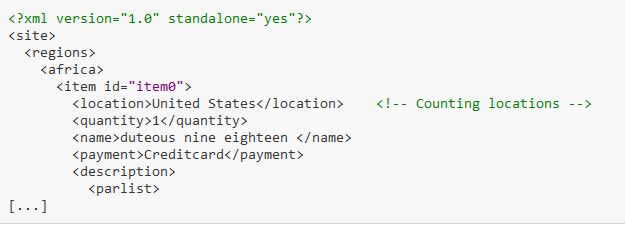
\includegraphics[width=0.75\textwidth]{figures/XML}}
	\caption{XML stream parsing dengan iterparse}
	\label{XML stream parsing dengan iterparse}
\end{figure}
